\documentclass[12pt]{article}
\usepackage{makeidx}
\makeindex
\usepackage{subcaption}
\usepackage[utf8]{inputenc}%acentuação das palavras
\usepackage[T1]{fontenc}%codificação de fonte
\usepackage[brazilian]{babel}
\usepackage{tikz}
\usepackage{textcomp}
\usepackage{afterpage}
\usepackage{varwidth}
\usepackage{indentfirst}
\usepackage{amsfonts}
\usepackage{amsmath}
\usepackage{amsthm}
%\usepackage{amssymb}
\usepackage{amscd}
\usepackage{amsxtra}
\usepackage{latexsym}
\usepackage{hyperref}
%\usepackage{cleveref}
\usepackage{enumerate}
\usepackage{fancyhdr}
\usepackage{etoolbox}
\usepackage{multicol}
\usepackage{multirow}
\usepackage{setspace} \onehalfspacing
\usepackage{mathptmx}
\usepackage[portuguese,ruled,vlined,linesnumbered]{algorithm2e}%algoritmos
\setlength{\parindent}{1.5cm}
\usepackage[a4paper,top=3cm,bottom=2cm,left=3cm,right=2cm,marginparwidth=1.75cm]{geometry}
\usepackage{lastpage}
\usepackage{fancyhdr}

\usepackage[italic]{mathastext}
\usepackage{graphicx}
\usepackage{longtable}

\title{Projeto 2 - MS960/MT862}
\author{Fernando Ribeiro de Senna --- RA 197019\\
Rodolfo}
\date{13 de novembro de 2020}
\begin{document}
\maketitle

Foi implementada rede neural regularizada para classificar dígitos manuscritos. Foram utilizados como exemplos de treinamento imagens provenientes da base de imagens MNIST ($20 \times 20$), linearizadas em vetores de 400 entradas. A implementação computacional foi feita em linguagem \textit{python} em três arquivos: \textit{functions.py}, que contém as funções utilizadas; \textit{neural\_networks\_p2\_1.ipynb}, que contém a parte 1 do projeto (mais voltada à implementação do algoritmo) e \textit{Avaliacao\_NeuralNet.ipynb} que contém a parte 2 do projeto (voltada à seleção de do modelo).

A Seção \ref{doc} apresenta documentação das funções implementadas no arquivo \textit{functions.py,} a Seção \ref{dados} apresenta a forma como foi feita a importação e o processamento dos dados (comum aos arquivos \textit{neural\_networks\_p2\_1.ipynb} e \textit{Avaliacao\_NeuralNet.ipynb}), a Seção \ref{parte1} versa sobre a implementação computacional da parte 1 do projeto e a Seção \ref{parte2} apresenta o que foi feito na parte 2 do projeto.

Foram utilizados funções e objetos das bibliotecas \textit{pandas, numpy} e \textit{matplotlib}. 

Toda a fundamentação teórica se baseia em conteúdo oferecido em vídeo-aulas e \textit{slides} pelo Professor João Batista Florindo em ocasião de oferecimento da disciplina MS960 no segundo semestre de 2020 pelo Instituto de Matemática, Estatística e Computação Científica (IMECC) da Universidade Estadual de Campinas (UNICAMP).


\section{Documentação} \label{doc}
Essa Seção apresenta as funções utilizadas no projeto, implementadas no arquivo \textit{functions.py.}

\subsection{Função backpropagation}
Função que realiza o treinamento da rede neural.

Argumentos de entrada:

\begin{description}
\item[X] Matriz com dados do conjunto de treinamento.

\item[y] Vetor com rótulos corretos para o conjunto de treinamento.

\item[num\_labels] (int) Número de rótulos (números) distintos no conjunto de treinamento.

\item[hidden\_layer\_size] Lista contendo o número de unidades de ativação em cada uma das camadas escondidas da rede neural.

\item[Lambda] (int) Valor de $\lambda$ a ser usado na regularização.

\item[alpha] (int) Taxa de aprendizado.

\item[nbr\_iter] (int) Número de iterações.

\item[regularizada] Booleano que indica se deve ser utilizada regularização ou não (opcional, padrão é \textit{True}).
\end{description}

A função retorna:

\begin{description}
\item[theta] Lista de \textit{arrays} contendo os valores dos parâmetros $\Theta$ obtidos pelo treinamento

\item[J\_history] Lista com os valores da função de custo para cada iteração
\end{description}

A função cria uma lista de \textit{arrays} inicializados aleatoriamente pela função \textit{randInitializeWeights} com dimensões coerentes com a arquitetura da rede neural fornecida pelo usuário. Em seguida, é realizado o treinamento utilizando a função \textit{gradientDescent}, obtendo, com isso, os argumentos de saída da função.

\subsection{Função computeCost}

\subsection{Função gradientDescent}

\subsection{Função prediction}

\subsection{Função randInitializeWeights}

\subsection{Função sigmoid}

\subsection{Função sigmoidGradient}

\subsection{Função zero\_col}
Função que remove colunas (de um \textit{dataframe}) em que todas as entradas são nulas.

Argumento de entrada:

\begin{description}
\item[df] \textit{Dataframe}
\end{description}

Argumentos de saída:
\begin{description}
\item[df] Matriz contendo os dados do \textit{dataframe}, após serem removidas as colunas em que só haviam zeros.

\item[zero\_cols] Lista contendo os índices das colunas removidas.
\end{description}

A função percorre o \textit{dataframe} verificando quais colunas são nulas, as remove e armazena seus índices em uma lista. Por fim, retorna o \textit{dataframe} (convertido em matriz e sem as colunas nulas) e a lista dos índices das colunas nulas.

\section{Importação e processamento dos dados} \label{dados}
Esse processamento de dados é comum a ambas as partes do projeto e está presente nos arquivos \textit{neural\_networks\_p2\_1.ipynb} e \textit{Avaliacao\_NeuralNet.ipynb}.

Para importação dos dados, foi utilizada a função \textit{read\_csv} da biblioteca \textit{pandas}, para importar as imagens do arquivo \textit{imageMNIST.csv} e os números a que correspondem do arquivo \textit{labelMNIST.csv.} Uma vez importados os dados, foi realizada remoção de dados excessivos.

No conjunto de exemplos de treinamento, havia alguns \textit{pixels} que apresentavam valor nulo para todas as imagens presentes no conjunto de treinamento. Assim, a fim de evitar a presença excessiva de atributos na rede neural, as colunas da base de dados correspondentes a essas imagens foram removidas, já que não interfeririam no resultado. Essa transformação é feita pela função \textit{zero\_col}.

Por fim, definem-se as variáveis X e y, que são, respectivamente, uma matriz em que cada linha representa os \textit{pixels} de uma imagem do conjunto de treinamento e um vetor com os rótulos corretos do conjunto de treinamento.

\section{Implementação do Algoritmo --- Parte I} \label{parte1}
As operações descritas nessa Seção estão no arquivo \textit{neural\_networks\_p2\_1.ipynb} e são relativas à primeira parte do projeto. A importação e o processamento dos dados foram feitos conforme descrito na Seção \ref{dados}.


\subsection{Visualização das unidades de ativação escondidas}
A fim de ser possível visualizar a contribuição de cada unidade de ativação escondida, foi representado gráficamente o vetor de parâmetros $\Theta^{(1)}$ (após realização do \textit{backpropagation}), que contém os parâmetros que "transportam" \ os dados de entrada para cada unidade de ativação da camada escondida.

Para isso, removeu-se o \textit{bias} de cada uma das linhas (cada linha corresponde a uma unidade de ativação) e acrescentaram-se os valores de $\Theta^{(1)}_{i,j}$ que correspondem aos \textit{pixels} que são nulos em todas as imagens e foram retirados dos exemplos de treinamento conforme discutido na Seção \ref{dados}. O valor desses parâmetros inseridos é zero, pois não contribuem com os resultados obtidos na base de dados utilizados.

Em seguida, os valores dos parâmetros foram normalizados a fim de facilitar a visualização. Para isso, utilizou-se (com relação a cada unidade de ativação) o processo de \textit{scaling}, em que cada valor é substituído pela divisão entre a diferença entre o valor e o valor mínimo e a diferença entre os valores máximo e mínimo, conforme pode ser visto na Equação \ref{scaling}.

\begin{equation} \label{scaling}
\Theta^{(1)}_{i,j} := \frac{ \Theta^{(1)}_{i,j} - \min\limits_i\left\{\Theta^{(1)}_{i,j}\right\}}{\max\limits_i\left\{\Theta^{(1)}_{i,j}\right\} - \min\limits_i\left\{\Theta^{(1)}_{i,j}\right\}}
\end{equation}

Por fim, cada linha de $\Theta^{(1)}_{i,j}$ é rearranjada em imagem de dimensão $20 \times 20$ \textit{pixels} e impressa com auxílio de funções da biblioteca \textit{matplotlib.} A Figura \ref{img_un_escond} apresenta a representação gráfica de cada uma das unidades de ativação escondidas após realizar treinamento com todas as 5 mil imagens do conjunto de treinamento através da função \textit{backpropagation} com uma camada escondida com 25 unidades de ativação, $\lambda = 0,001, \ \alpha = 0.8$ e 800 iterações.

\begin{figure}
\begin{center}
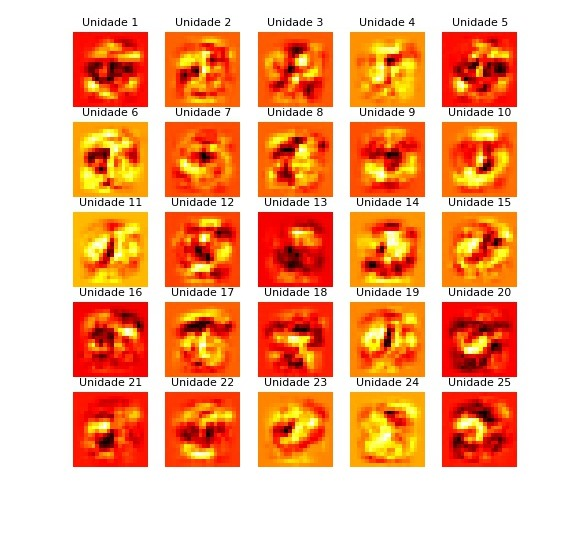
\includegraphics[scale=0.8]{corte_unidades_ativacao.jpg}
\caption{Representação gráfica das unidades de ativação da camada escondida.} \label{img_un_escond}
\end{center}
\end{figure}

\section{Seleção de modelo --- Parte II} \label{parte2}
As operações descritas nessa Seção estão no arquivo \textit{Avaliacao\_NeuralNet.ipynb} e são relativas à segunda parte do projeto. A importação e o processamento dos dados foram feitos conforme descrito na Seção \ref{dados}.


\subsection{Treino, validação e teste} \label{treino, val, teste}
\indent Inicialmente, os 5 mil exemplos de treinamento foram separados em 3 conjuntos distintos: treino, validação e teste, com 60\%, 20\% e 20\% do total de exemplos, respectivamente. Essa divisão foi feita de forma aleatória, utilizando a função \textit{random.permutation} da biblioteca \textit{numpy}.

A fim de garantir que não haveria desbalanceamento de classes, isto é, que um conjunto contivesse mais imagens correspondentes a um número do que a outro, essa separação aleatória foi feita classe a classe, de modo que no fim, 60\% dos exemplos referentes a cada número estivesse no conjunto de treino, 20\% no de validação e 20\% no de teste.

Uma vez separados os exemplos de treinamento nesses três conjuntos, realizou-se treinamento utilizando o conjunto de treino e a função \textit{backpropagation} com 800 iterações, $\alpha = 0,8$ e $\lambda=0,001$ (valor obtido através dos testes da Seção \ref{lambda_otimo}). Em seguida, verificou-se o desempenho do resultado para os conjuntos de treino, validação e teste. O algoritmo classificou corretamente 94,57\% das imagens do conjunto de treino, com função de custo avaliada em 0,4115. Foram classificadas corretamente 91,8\% das imagens do conjunto de validação, obtendo 0,5556 para o valor da função de custo. Já para o conjunto de teste, foram classificadas corretamente 90,7\% das imagens, com função de custo 0,5832.

Como os resultados do primeiro treinamento foram satisfatórios ao serem aplicados aos conjuntos de validação e teste, foi feito novo treinamento, dessa vez utilizando tanto o conjunto de treino quanto o de validação. Novamente, foram utilizadas 800 iterações, $\alpha = 0,8$ e $\lambda=0,001$. Para os conjuntos de treino e validação (conjunto de exemplos de treinamento desse novo treinamento), o algoritmo classificou corretamente 94,77\% das imagens, com função de custo avaliada em 0,4173. Já para o conjunto de teste, foram classificadas corretamente 91,6\% das imagens, com 0,5455 como valor para a função de custo.

Conforme esperado, houve pouca variação no desempenho para o conjunto utilizado como treinamento nos dois casos, uma vez que os hiperparâmetros foram os mesmos. Além disso, para o conjunto de teste, o desempenho do algoritmo de classificação foi melhor, pois havia mais exemplos de treinamento quando a rede neural foi treinada, melhorando a precisão.

\subsection{Curvas de aprendizado}
Curvas de aprendizado são gráficos que servem para comparar o desempenho dos conjuntos de treino e validação para diferentes quantidades de exemplos de treinamento. Para construí-las, é necessário realizar diversos treinamentos, cada um com uma quantidade diferente de exemplos de treinamento e comparar os erros do conjunto utilizado para treinamento e o conjunto utilizado para validação.

Para construir essas curvas, foram utilizados os conjuntos de treino e validação descritos na Seção \ref{treino, val, teste}. Foram realizados 30 treinamentos, com $100, 200, \ldots, 3000$ exemplos do conjunto de treino, garantindo que em nenhum treinamento houvesse desbalanceamento de classes. Nesses treinamentos, foram usados $\lambda=0,001, \ \alpha=0,8$ e 800 iterações. Em seguida, construiu-se o gráfico das curvas de aprendizado, com o valor do erro dos conjuntos de treino (somente as amostras usadas naquele treinamento) e validação em função do tamanho do conjunto usado no treinamento. O resultado está na Figura \ref{curvas_aprendizado}.

\begin{figure}
\begin{center}
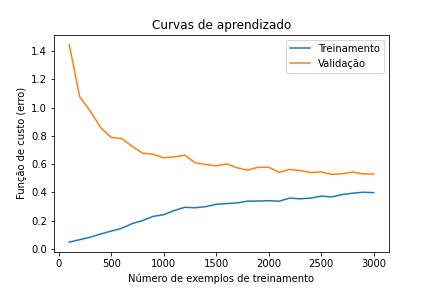
\includegraphics[scale=0.8]{curvas_aprendizado.jpg}
\caption{Curvas de aprendizado.} \label{curvas_aprendizado}\end{center}
\end{figure}

Conforme esperado, o erro do conjunto de treinamento se torna cada vez maior, devido à maior quantidade de exemplos, enquanto para o conjunto de validação o erro diminui, de forma a torná-los cada vez mais próximos. 

\subsection{Seleção de $\lambda$} \label{lambda_otimo}
Nessa Seção, é descrito o procedimento utilizado para encontrar o valor ótimo de $\lambda$ na regularização. Para isso, foram feitos dez treinamentos com o conjunto de treino, todos com 800 iterações e $\alpha=0,8$, variando o valor de $\lambda$ no conjunto $\{0; 0,001; 0,003; 0,01; 0,03; 0,1; 0,3; 1; 3; 10\}$. Para cada treinamento, avaliou-se o erro para o conjunto de validação.

Para analisar o resultado, foram construídos três gráficos:  evolução do erro do conjunto de validação em função de $\lambda$ (Figura \ref{evolucao_lambda}),  evolução do erro do conjunto de validação com relação ao $\lambda$ para os primeiros 6 treinamentos (Figura \ref{primeiros_lambda}) e logaritmo do erro em função do logaritmo de $\lambda$ (Figura \ref{log_lambda}). Os três gráficos são úteis para visualizar o resultado, pois, devido à grande variação de $\lambda$, apenas um deles é insuficiente para perceber os resultados adequadamente.

\begin{figure}
\begin{center}
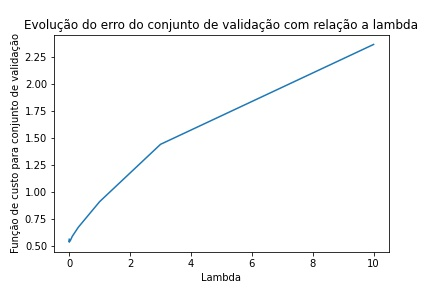
\includegraphics[scale=0.8]{evolucao_lambda.jpg}
\caption{Evolução da função de custo para o conjunto de validação em função de $\lambda$.} \label{evolucao_lambda}
\end{center}
\end{figure}

\begin{figure}
\begin{center}
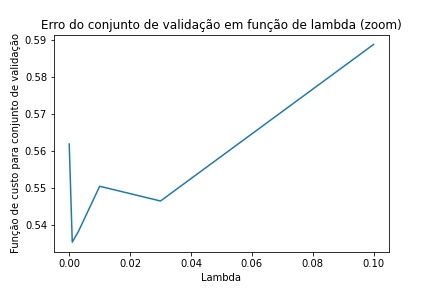
\includegraphics[scale=0.8]{primeiros_lambda.jpg}
\caption{Evolução da função de custo para o conjunto de validação em função dos seis primeiros valores de $\lambda$.} \label{primeiros_lambda}
\end{center}
\end{figure}

\begin{figure}
\begin{center}
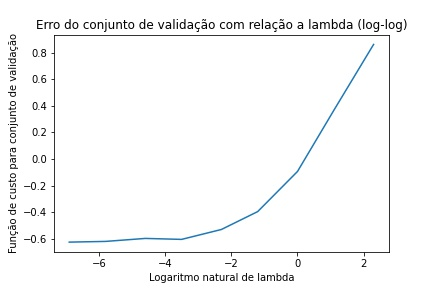
\includegraphics[scale=0.8]{log_lambda.jpg}
\caption{Evolução do logaritmo da função de custo para o conjunto de validação em função do logaritmo de $\lambda$.} \label{log_lambda}
\end{center}
\end{figure}

A partir dos resultados desses treinamentos e da comparação com o desempenho do conjunto de validação, obteve-se 0,001 como valor ótimo para $\lambda$. Com base nesse resultado, novo treinamento foi realizado, dessa vez usando tanto o conjunto de treino quanto o de validação como exemplos, utilizando 800 iterações, $\alpha=0,8$ e $\lambda=0,001$. Avaliou-se, então, o desempenho do método ao aplicá-lo ao conjunto de teste, obtendo classificação correta para 91,6\% das imagens e função de custo avaliada em 0,5319.


\section{Referências}
Vídeo-aulas e \textit{slides} pelo Professor João Batista Florindo em ocasião de oferecimento da disciplina MS960 no segundo semestre de 2020 pelo Instituto de Matemática, Estatística e Computação Científica (IMECC) da Universidade Estadual de Campinas (UNICAMP).


\end{document}